\documentclass[12pt]{article}

\usepackage[utf8]{inputenc}
\usepackage[a4paper,top=2.1cm,bottom=2.1cm,left=2.4cm,right=2.4cm]{geometry}
\usepackage{graphicx}
\usepackage{setspace}
\usepackage{tabularx}
\usepackage{xcolor}
\usepackage{amsmath}
\usepackage{amssymb}
\usepackage[backend=biber,style=numeric]{biblatex}
\usepackage[pdfpagelabels]{hyperref}
\usepackage{mdframed}
\usepackage{subcaption}

\addbibresource{main.bib}

% custom commands
\newcommand{\todo}[1]{{\color{red}#1}}
\newcommand{\comment}[1]{}
% shorthand command aliases
\newcommand{\fancy}{\mathcal}

\begin{document}

\begin{titlepage}
       \Large
       \begin{center}
           
\includegraphics[width=0.4\textwidth]{imgs/logo.png}
       \end{center}
       \renewcommand{\thepage}{Title}
       \thispagestyle{empty}
          \begin{center}
              \vspace*{1cm}
       \linespread{1.25}
              {\doublespacing \Huge\textbf{$\epsilon$-Differential Privacy and Low-Population Histogram Estimation}}
       \linespread{1}
              \vspace*{0.5cm}
              \rule{\linewidth}{1pt}
              \vspace*{1em}
              {\huge Bachelor Thesis \\
              \Large Department of Mathematics and Computer Science, \\
              University of Southern Denmark}
       \end{center}
       \vspace{2cm}
       \Large
       \begin{tabularx}{\textwidth}{lXr}
           Author & & Johan Fagerberg \\
           Supervisor & & Jacopo Mauro \\
       \end{tabularx}
       
       \vfill
       \begin{center}
           \large \today
       \end{center}
       \end{titlepage}


\renewcommand{\abstractname}{Abstract}
\begin{abstract}
\todo{Todo}
\end{abstract}

\begin{center} \bf Keywords \end{center}

\thispagestyle{empty}
\tableofcontents
\newpage

\section{Introduction}

Privacy-preserving data collection has long been an area of interest for many, but never before has it seen as significant focus as it has over the last few decades. With the advent of the Internet, and the global shift towards highly connected lifestyles that comes with it, data can now be gathered from almost every aspect of our lives---and with that comes a need to guarantee subject privacy.

For a long time this has been attempted primarily through techniques that ``anonymizes'' incoming data, attempting to remove any information that may lead to privacy loss. Unfortunately this approach has shown itself to be fallible: without formal guarantees, it relies on the foresight of the data analysts who decides what data to remove, which often leads to de-anonymization when auxiliary data---or simply insufficient anonymization---is present.

\bigskip

Historically it has been particularly challenging to provide formal guarantees in the ``non-interactive'' setting\footnote{As opposed to the ``interactive'' setting, where the data collector keeps the data set private, but allows users to query the data in some limited way.}, where data sets are published publicly after some form of anonymization. In this setting the primary defense has been the removal of known identifiers, such as names and birthdates, or other limitation of information from the data set through techniques like sub-sampling. These approaches have seen widespread use, including in particularly sensitive areas like health data, but have repeatedly fallen under re-identification attacks (see e.g. \cite{reidentification2011}).

In recent years, an alternative approach has emerged in the form of \emph{differential privacy}. The culmination of a line of research explored in \cite{precursor_2003,precursor_2004,precusor_2005}, Dwork et al. formalize the concept in \cite{dworketal2006} by introducing their formal description of ``privacy loss''. Differential privacy not only offers a way to describe and compare differentially private algorithms, but also guarantees that the privacy provided by such algorithms does not falter in the presence of unforeseen auxiliary information or attack approaches.

Differential privacy has since been subject to considerable interest. It has seen numerous high-profile applications, including the 2020 US census \cite{us_census}, as well as data gathering from companies like Apple \cite{apple_differential,apple_differential_loss}, Google \cite{google_rappor,google_prochlo} and Microsoft \cite{dworketal2006,microsoft_telemetry}. Even beyond its roots in cryptography and statistics it has also found application in areas like machine learning \cite{ml_abadi,ml_shokri,ml_papernot}. With the growing focus on digital data collection and the privacy concerns that follow, differential privacy has become an important tool for academics and companies alike.

\bigskip

In this thesis we will be exploring the definition of differential privacy, the guarantees it provides (and which ones it doesn't), and how common statistical problems are solved in differentially private ways. Finally, we will be exploring one particular algorithm for differentially private histogram estimation in the local setting \cite{microsoft_telemetry}, and evaluate its performance in low-population scenarios.

\section{Differential privacy \label{sec:diffpriv}}

\subsection{Motivation \label{sec:motivation}}

Before exploring the concept of differential privacy, it is worthwhile to spend some time understanding the problem that it aims to solve. \bigskip

As data scientists, we often want to guarantee subjects (meaning the people whose responses our database is built from) that no ``private data'' can be leaked. This is especially important when working with sensitive data, like medical histories or crime statistics, where the consequences of privacy breaches are significant.

Giving such a guarantee naturally requires defining what it means to reveal ``private data''. Intuitively we have to balance our interest in interesting research with our interest in protecting subject privacy: we cannot reveal \emph{nothing}, as that would make it impossible to conclude anything worthwhile, but we also cannot reveal too much, as that would violate our promise of privacy. The question then is: what can (and can't) we reveal?

The common distinction is made between data that enables identification of the subjects, and data that doesn't. This builds on the intuition that a subject's privacy specifically relates to knowing something about \emph{them}, and cannot be harmed without some link between them and the data.

Consider the example of a smoker who participated in a study related to lung cancer: if the database of the study is released unmodified, it will be trivial for anyone to determine whether they had lung cancer, which would certainly be considered a breach of privacy. If the database is modified in such a way that no participant can be identified, it might be possible to determine that \emph{someone} had lung cancer, but not who it was. In order for the database to be useful, it must also be possible to draw interesting conclusions (such as a link between smoking and lung cancer) from the database, despite the anonymization efforts. It is interesting to note that this enables people who already know that the subject is a smoker to learn something new about them (such as that they have an increased risk of lung cancer), but that we do not consider this a breach of privacy---in fact this could be learned even if the subject \emph{hadn't} participated in the study. \bigskip

Historically the privacy guarantees given by various anonymization techniques have been much more limited than the one described above, protecting primarily against specific and limited attacks. It has been particularly difficult to protect subject privacy in the so-called ``non-interactive'' setting, where data sets are published publicly after some form of anonymization. Unlike the interactive setting, where the data controller is the one responding to queries, and therefore is able to make decisions based on the specific queries made, this setting requires strong generalized anonymization. The primary defense has long been the removal of known identifiers, such as names and birthdates, or other limitation of information from the data set through techniques like sub-sampling.

The problem with these defenses is that they are often vulnerable to unforeseen auxiliary data, and they cannot be generalized across different projects. Although the removal of birthdates and names may be sufficient for one use case, that doesn't mean they are generally sufficient: in fact there have been numerous real-world examples where data scientists have released what they believed to be ``anonymized'' data sets, ranging from medical records to social networking data, just to have them be successfully de-anonymized by researchers (see e.g. \cite{reidentification2011}).

Consider the previous example of a smoker participating in a study related to lung cancer. The data collector may argue that by aggregating the data by age groups, such that the only information released is how many subjects in each age group tested positive for lung cancer, each individual subject are protected against identification. Nonetheless, a neighbor may know that the subject is participating in the study, be able to observe on which days they leave for the hospital, and know that the study releases updated statistics frequently. Armed with this auxiliary information, even the previously innocuous-seeming aggregate information may be enough to make an educated guess, or even identify, whether the subject in question has been diagnosed with lung cancer by simply observing changes in the expected age group. \bigskip

An alternative approach that has regained popularity in the last 20 years is based on perturbing the data by introducing noise.

A classic example is that of randomized response, where subjects are asked to answer randomly to some degree: prior to answering some sensitive yes/no question they are asked to flip a coin. If the coin lands on heads, they should answer truthfully. If not, they should answer ``yes''\footnote{Or ``no'' if that is the sensitive option. In some variants they are asked to flip a second coin and answer ``yes'' if it lands on heads, ``no'' otherwise.}. In this way subjects have a degree of \emph{plausible deniability}---even if they answered ``yes'' to a sensitive question, they can later claim that that coin simply landed on tails. The data collector is nonetheless able to calculate the expected proportion of respondents with each true answer using simple mathematics (although with significant uncertainty for small survey sizes).

This intuition can be extended further, and combined with other approaches. Take the example from earlier, where a neighbor was able to guess whether a subject had lung cancer by observing aggregate statistics. Had the data collector added noise to those statistics, the neighbor would have no way of knowing whether an increase in the number of subjects with lung cancer was a result of an actual diagnosis, or merely the result of the noise---assuming the noise was correctly applied. \bigskip

With so many different ways to implement privacy, a natural question is ``how---and how much---should we perturb our data in order to protect subject privacy adequately''. It is this question that differential privacy aims to provide a way to answer.

\subsection{Differential privacy \label{sec:promise}}

Differential privacy was formalized in 2006 by Dwork et al. \cite{dworketal2006}, following a line of research into privacy provided by noise-perturbation of data sets \cite{precursor_2003,precursor_2004,precusor_2005}. It tackles the problem of how we can mathematically guarantee that the privacy of a subject cannot be breached by the output of some algorithm (i.e. a process that takes our data set and provides an output)---and how we can design algorithms that provide such guarantees.

The notion of privacy introduced in the paper relies on the intuition that an algorithm cannot violate the privacy of someone whose data isn't used in it. If the output of the algorithm didn't depend at all on a particular subjects data, then the output cannot breach said subjects privacy. If we could provide this guarantee to all of our subjects, then the algorithm wouldn't be a privacy risk at all.

This guarantee is unfortunately impossible to provide to all subjects. As proven by Dwork in the follow-up paper \cite{dwork2006_diffpriv}, revealing nothing about any subject while still providing utility is impossible. If we were to give this guarantee to each of our subjects, then we could not learn anything from our data set, rendering it useless. Instead, we can promise our subjects that the influence of their data on the output is \emph{almost} none---that the likelihood of seeing each possible output is almost the same with or without their data. This guarantee still gives them a strong degree of privacy through plausible deniability, depending on our definition of ``almost''. \bigskip

Consider the example from earlier, with a subject participating in a study related to lung cancer. A third party may wish to use our output to learn something about the subject, in breach of the subjects privacy. With our guarantees it is very limited what they can learn: even if they see an output that indicates that the subject had lung cancer, they are almost as likely to see that output if the subject didn't have lung cancer. No matter the output, the certainty with which they can come to a conclusion one way or the other is limited by our guarantees.

It's important to note that this doesn't mean that the third party can't learn \emph{anything} about our subject. If they're interested in information that doesn't depend on the subjects specific response---e.g. whether the subjects age group has a heightened risk of lung cancer---then our privacy guarantee does not protect this information. We only consider it a privacy breach if they can learn something that they wouldn't have been able to learn if the subject hadn't participated in the study. \bigskip


This leads us to our definition of differential privacy, here formulated as done by Dwork in \cite{dwork2006_diffpriv}:

\begin{mdframed}
    \textbf{Differential privacy:} Given an algorithm $\fancy{K}$, we say that it provides $\epsilon$-differential privacy if for any two data sets $D_1$ and $D_2$ differing on at most one element, and any $S \subseteq \text{Range}(\fancy{K})$, it holds that
    \begin{equation}\label{eq:diffpriv}
        \Pr[\fancy{K}(D_1) \in S] \leq \exp(\epsilon) \cdot \Pr[\fancy{K}(D_2) \in S]
    \end{equation}
\end{mdframed}

This definition is simple, but important in many ways.

Most importantly, it gives us a formal measure for just how private an algorithm is. The $\epsilon$ parameter describes just how close two probabilities have to be for us to consider them ``almost'' unchanged. This means that we are able to compare algorithms, even across problem statements, on how well they protect subject privacy. We are able to describe the effect that changes, such as composition with other algorithms, have on the privacy guarantees provided by an algorithm---in many cases this can even be done generally, giving us composition theorems that hold for any $\epsilon$-differentially private algorithm.

Having such formal measures further allows us to communicate the guarantees given by our algorithms in concrete terms. Going from vague best effort guarantees to concrete and formally proven privacy protection is a big win for subject privacy. It allows subjects to compare and evaluate surveys based on a simple measurement; this is especially important in a world where privacy is becoming a bigger and bigger topic in the public discourse, while systems processing data are becoming more and more complex. Having formal guarantees also helps the legislative enforcement of privacy-preservation that is becoming prevalent in some parts of the world, a process that has historically been difficult and vague as a result of poor formal definitions. \bigskip

An interesting effect of this privacy definition is that a differentially private algorithm may not have any outputs that are only possible if a subject has given a particular answer. Each output in the range of the algorithm \emph{must} have a non-zero probability, no matter the true data set. This hints at the common implementation technique of perturbing either the data or output with noise, which we will explore more in section \ref{sec:achieving}.

\subsubsection{The privacy parameter $\epsilon$ \label{sec:epsilon}}

At the core of our definition is the $\epsilon$ parameter. This describes how much a single entry can affect the output probabilities for us to consider them ``almost'' unchanged, with high values permitting high privacy loss, and low values protecting subject privacy well. It is often known as the ``privacy measure'' or ``privacy parameter'', as it allows us to directly compare the privacy guarantees provided by two differentially private algorithms.

Which values we consider reasonable for $\epsilon$ depends on the specific usage scenario in question. For particularly sensitive data, where we want third parties to be unable to determine a subjects response with any reasonable certainty, we may want $\epsilon$ values less than 1. For less sensitive data we may find higher values, sometimes as high as 10, acceptable. It is important to note that as $\epsilon$ is used as an exponent in definition \ref{eq:diffpriv}, the privacy guarantees quickly degrade as $\epsilon$ increases---a 10-differentially privacy algorithm allows for an output to be 22000 times more likely given a specific subjects response, while a 2-differentially private algorithm only allows a factor of 7.

The privacy parameter $\epsilon$ is also often called the ``privacy budget''. As we will see in section \ref{sec:composition}, combinations of differentially private algorithms often lead to differentially private algorithms whose $\epsilon$ depends on the $\epsilon$ of the combined algorithms. If we define a global $\epsilon$ value, describing the privacy loss we are willing to accept for our subjects, then we are able to pick algorithms that each ``use'' a part of this privacy budget. This notion of $\epsilon$ as a budget for algorithms to be limited allows us to design our algorithms with the privacy guarantees in mind from the very beginning.

It is often the case for differentially private algorithms that low values of $\epsilon$, which provide good privacy protection, also degrades the utility of the output. If the algorithm masks the contribution of subjects using noise, then more noise is required as $\epsilon$ decreases, leading to less accurate results. For this reason there is often an inherent balancing act when it comes to differential privacy: low values of $\epsilon$ provide good privacy, but poor data utility, while high values of $\epsilon$ provides the inverse. As such, finding an $\epsilon$ value that is acceptable both in terms of privacy and data utility is crucial. Common values for large commercial data sets \cite{apple_differential,us_census} are in the range of 4-6, but since commercial data collectors are often incentivized to prioritize utility over subject privacy, it is important that each subject is able to evaluate the $\epsilon$ values of a given study and decide for themselves whether they are satisfactory. \bigskip

It is important to note that, although $\epsilon$ allows us to compare the privacy guarantees offered by two algorithms directly, we must be careful in the conclusions we draw. In particular, we are not able to compare algorithms for simply failing to reach a certain degree of differential privacy: an algorithm that is not $\epsilon$-differentially private for some $\epsilon$ may simply be $2\epsilon$-differentially private, which is almost identical for low values of $\epsilon$. Another algorithm failing to achieve the same $\epsilon$-differential privacy may release the data set unaltered.



\subsection{Attributes and composition theorems \label{sec:composition}}

One of the great aspects of our definition of differential privacy is that we can formally describe attributes for algorithms, and how their privacy guarantees are affected by changes such as composition---and that we are able to do this generally, and not just for one specific algorithm.

\subsubsection{Immunity to post-processing}

One such attribute that we are able to formally prove is that of \emph{immunity to post-processing}. Recall our example from section \ref{sec:motivation}, where a neighbor was able to make an educated guess at whether a subject had lung cancer based on auxiliary data. This was an informal example of post-processing: the third party was able to combine auxiliary data with the survey output, and process it into a data set that violated the subject's privacy to a higher degree than the survey output on its own did. It is fairly simple to show that post-processing leading to privacy loss is \emph{not} possible for the output of differentially private algorithms (assuming the true data set is kept secret), as done in \cite{dwork_privacybook}:

Let us imagine an $\epsilon$-differentially private algorithm $\fancy{K} : X \to R$. For any post-processing function $f : R \to R'$, we can show that the algorithm $f \circ \fancy{K}$ is also $\epsilon$-differentially private---that is, there are no post-processing functions that increase the privacy loss of the original algorithm. For any two neighboring data sets $D_1$ and $D_2$, and any event $S \subseteq R'$, we define $T = \{r|f(r) \in S\}$ to be the outputs of $\fancy{K}$ that lead to event $S$. Then we have
\begin{align*}
    \Pr[\fancy{K}(D_1) \in T] &= \Pr[f(\fancy{K}(D_1)) \in S]  \\
    &\leq \\
    \exp(\epsilon)\cdot\Pr[\fancy{K}(D_2) \in T] &= \exp(\epsilon)\cdot\Pr[f(\fancy{K}(D_2)) \in S],
\end{align*}
where the inequality follows from definition \ref{eq:diffpriv}. This shows that $f \circ \fancy{K}$ is also $\epsilon$-differentially private, if $f$ is deterministic. It can be extended to non-deterministic functions \todo{as these can be decomposed into a convex combination of deterministic functions, and convex combinations preserve differential privacy}.

It is important to note that this proof fails if $f$ has knowledge of the original data set. In this case the equalities do not hold, meaning the result is not necessarily $\epsilon$-differentially private. The immunity to post-processing therefore only holds when the input to $\fancy{K}$ is kept private. \bigskip

This proof is crucial because it formalizes and important aspect of our privacy guarantee. With this immunity we know that our guarantee cannot be compromised or harmed after we release our data, by anyone who does not have access to our original data set---unlike many other anonymization techniques that can often be de-anonymized later as unexpected auxiliary data becomes available. If the data set is properly anonymized using differential privacy, and the original data set is discarded, then our privacy guarantees will hold perpetually, regardless of new techniques or auxiliary data being discovered.

\subsubsection{Group privacy}

Another important attribute of differentially private algorithms is that the privacy guarantee readily extends to groups of subjects. There are cases where we may wish to describe how our guarantee holds for groups of subjects, e.g. families, so as to ascertain how much privacy loss the group as a whole can suffer.

Formally this would mean describing how our probabilities change for any two data sets $D_0$ and $D_k$ that differ in at most $k$ entries, where $k$ is the size of the group we are interested in. By constructing data sets $D_0, D_1, \dots, D_k$ such that data sets $D_i,D_j$ differ in at most $|i-j|$ entries, we can see from definition \ref{eq:diffpriv} that
\begin{align*}
    \Pr[\fancy{K}(D_0) \in S] &\leq \exp(\epsilon) \cdot \Pr[\fancy{K}(D_1) \in S] \\
        &\leq \exp(\epsilon) \cdot \exp(\epsilon) \cdot \Pr[\fancy{K}(D_2) \in S] \\
        &\qquad\vdots \\
        &\leq \exp(\epsilon)^k \cdot \Pr[\fancy{K}(D_k) \in S] = \exp(k\epsilon) \cdot \Pr[\fancy{K}(D_k) \in S].
\end{align*}

This shows that any $\epsilon$-differentially private algorithm is $k\epsilon$-differentially private for groups of size $k$. \bigskip

Note that this means that the $\epsilon$ value for the group algorithm is linearly dependent on the size of the group. As $\epsilon$ is an exponent in definition \ref{eq:diffpriv}, this means that our privacy guarantees quickly degrade as $k$ increases, requiring the same considerations as those described in section \ref{sec:epsilon}.

\subsubsection{Linear combinations of differentially private algorithms}

There are cases where we may wish to employ two differentially private algorithms on the same data set, and release both outputs. This scenario can be modelled as the combined algorithm $\fancy{K}_{1,2}(x)=\left(\fancy{K}_1(x), \fancy{K}_2(x)\right)$, where $\fancy{K}_1$ is $\epsilon_1$-differentially private, and $\fancy{K}_2$ is $\epsilon_2$-differentially private. It can be shown that $\fancy{K}_{1,2}$ is then $\epsilon_1+\epsilon_2$-differentially private.

The proof of this is again rather simple. For any two data sets $D_1,D_2$ differing in at most one entry, and any $(r_1,r_2) \in \text{Range}(\fancy{K}_{1,2})$, we have
\begin{align*}
    \Pr[\fancy{K}_{1,2}(D_1)=(r_1,r_2)] &= \Pr[\fancy{K}_1(D_1)=r_1]\cdot\Pr[\fancy{K}_2(D_1)=r_2] \\
        &\leq \exp(\epsilon_1) \Pr[\fancy{K}_1(D_2)=r_1] \cdot \exp(\epsilon_2) \Pr[\fancy{K}_2(D_2)=r_2] \\
        &= \exp(\epsilon_1 + \epsilon_2) \cdot \Pr[\fancy{K}_1(D_2)=r_1] \cdot \Pr[\fancy{K}_2(D_2)=r_2] \\
        &= \exp(\epsilon_1 + \epsilon_2) \cdot \Pr[\fancy{K}_{1,2}(D_2)=(r_1,r_2)],
\end{align*}
showing that $\fancy{K}_{1,2}$ is $\epsilon_1+\epsilon_2$-differentially private.

This proof naturally extends to any number of combined algorithms. The combined algorithm $\fancy{K}_{1,2,3}(x)=\left(\fancy{K}_1(x), \fancy{K}_2(x), \fancy{K}_3(x) \right)$ can be modelled as $\fancy{K}_{1,2,3}(x)=\left(\fancy{K}_{1,2}(x), \fancy{K}_3(x)\right)$, and is thus $\epsilon_1 + \epsilon_2 + \epsilon_3$-differentially private---and this can be extended indefinitely. The algorithm $\fancy{K}_{[k]}(x)=\left(\fancy{K}_1(x), \dots, \fancy{K}_k(x) \right)$ is therefore $\sum_{i=1}^k \epsilon_i$-differentially private, if each $\fancy{K}_i$ is $\epsilon_i$-differentially private. \bigskip

This result is valuable to us. It tells us that we can combine differentially private algorithms without any further work or considerations. Simply releasing the outputs of each algorithm is in itself differentially private, and we can describe precisely how much privacy loss this incurs.

This is also an example of a composition theorem that allows us to practically apply the ``privacy budget'' philosophy as described in section \ref{sec:epsilon}. If the total work we perform on a data set is described by a set of $n$ differentially private algorithms, where we release the output of each, then this combination theorem tells us how high the $\epsilon$ value may be for each algorithm before we exceed our budget. \bigskip

This combination theorem is the only composition theorem we will show for $\epsilon$-differential privacy. More advanced composition theorems exist for the differential privacy variant known as $(\epsilon,\delta)$-differential privacy which we will explore in section \ref{sec:variant_eps_delta}. These further composition theorems are beyond the scope of this thesis, but interested readers may refer to \cite[ch.~3]{dwork_privacybook}.

\subsection{Achieving differential privacy \label{sec:achieving}}

\begin{description}
    \item[Laplace] For numeric functions (i.e. $f : \mathbb{N}^n \to \mathbb{R}^k$) we can make them differentially private by adding suitable noise to their output. The Laplace mechanism is one way of doing this.
    
    An important measure is the $\ell_1$-sensitivity of the function, defined as
    \begin{equation}
        \Delta f = \underset{\begin{subarray}{c}
            x,y \in \mathbb{N}^{n} \\
            ||x-y||_1 = 1
        \end{subarray}}{\max} || f(x)-f(y) ||_1,
    \end{equation}
    i.e. the biggest difference any one entry can have on the output. Intuitively we could mask the contribution of any one entry by adding noise of this size.
    
    Another important definition for the Laplace mechanism is the Laplace distribution, whose density function is defined as
    \begin{equation}
        \text{Lap}(b,x) = \frac{1}{2b} \exp \left( -\frac{|x|}{b} \right).
    \end{equation}
    
    Using this we can define create our $\epsilon$-differentially private function as
    \begin{equation*}
        f'(x) = f(x) + (Y_1, \dots, Y_k)
    \end{equation*}
    where $Y_i$ are independent random variables drawn from $Lap(\Delta f/\epsilon)$.
    
    \item[Exponential] The exponential mechanism is used for cases where the task is to choose the ``best'' response out of multiple choices. It does not add noise to the output, but rather 
\end{description}

\subsection{Variants of differential privacy}

\subsubsection{$(\epsilon, \delta)$-differential privacy \label{sec:variant_eps_delta}}

\begin{description}
    \item[$(\epsilon, \delta)$-differential privacy] The guarantee of $\epsilon$-differential privacy is strong. In some cases it may be practical to weaken our guarantee a bit, e.g. to allow rare events to impact our output beyond what would be allowed normally.
    
    A variant of differential privacy, called $(\epsilon, \delta)$-differential privacy \cite{dwork2006_delta_diffpriv}, alters the definition slightly, such that for any two neighboring data sets $D_1$ and $D_2$,
    \begin{equation}
        \Pr[\fancy{K}(D_1) \in S] \leq \exp(\epsilon) \cdot \Pr[\fancy{K}(D_2) \in S] + \delta.
    \end{equation}
    
    This definition allows algorithms that may not live up to the stronger guarantee of $\epsilon$-differential privacy (or which have large $\epsilon$ measures under that definition) to provide this weaker guarantee instead.
    
    This guarantee differs in some significant ways from the one provided by $\epsilon$-differential privacy. It allows the differential privacy guarantee to ``fail'' sometimes, giving outputs that---in the worst case---leak the presence (or absence) of the entry in question. For example, it allows the algorithm to have an output that \emph{never} happens, unless a particular entry is present---in which case it has a probability of at most $\delta$. If such an output is given, an attacker will know for certain that the entry is present.
    
    This is naturally undesirable. As such, low $\delta$ values are desired for $(\epsilon, \delta)$-differentially private algorithms, as this limits the likelihood of our privacy guarantee ``failing''. It is worth noting that the desirable range for $\delta$ depends on the population size. The likelihood of of a ``failure'' is at most $\delta$ for each entry in the data set. As this guarantee is given independently for each entry, the expected probability of ``failure'' for any of our $n$ entries is $\delta \cdot n$---since we do not want this to happen, our $\delta$ must generally be smaller if we work on larger data sets.
    
    \item[Local differential privacy] Also known as ``randomized response''. Indicates that the perturbation of data is done client-side, such that nothing can be learnt about a subjects true answer even with full knowledge of the individuals reported answer.
\end{description}

\section{Experiments with low-population telemetry collection \label{sec:telemetry}}

\subsection{Introduction}

A 2017 paper building on a local differentially private algorithm for repeatedly collecting metrics from subjects. Historically an issue has been that privacy guarantees quickly degrade over repeated collections, e.g. when collecting telemetry over time.

\subsection{Introduction/Historical context}

\subsection{Low population experiments}

\begin{description}
    \item[Experiment setup] We wish to explore the effect of low population size on the utility of the mean and histogram estimation mechanisms described in \cite{microsoft_telemetry}. The paper tests the estimation errors of population sizes varying from $0.3\times10^6$ to $3\times10^6$, but does not test the errors for lower population sizes than this; this leaves many applications---such as telemetry collection by smaller companies than Microsoft---with little information on the applicability of the mechanisms.
    
    We test both estimation mechanisms on synthetic data sets sampled from constant, uniform and (truncated) normal distributions, similar to those used in the empirical evaluation in the paper.
    
    \item[Mean estimation]
    
    \item[Histogram estimation]
    We aim to measure the \emph{histogram error} of the estimated histograms, defined as $\max_{v\in[k]} |\hat{h}(v)-h(v)|$ where $\hat{h}(v)$ is the estimated frequency of the bucket $v$, and $h(v)$ is the true frequency. This is the error measure used in the paper. In addition to this we also measure the Wasserstein distance between the true and the estimated histograms (with any negative values in the estimated histogram truncated to 0). The histogram error is used to measure the maximum error of any one bucket in the histogram. The Wasserstein distance is used to measure the distance of the entire histogram to the true values.
    
    In order for our results to be comparable to those of the original paper, we use similar parameters beyond the population size: we use $k=32$ evenly sized buckets on the range $[0,24]$, permanent memoization for repeated collection, but no output perturbation. We vary population size in the range $[10^3, 3\times10^5]$ and $\epsilon$ in the range $[0.1, 10]$. In order to minimize the impact of the random nature of the mechanisms, we calculate the metrics by averaging over 10 separate estimations.
    
    The results can be seen in figure \ref{fig:histogram_errors}. As expected, low population sizes give significantly worse estimation errors: at $n=10^4$ and $\epsilon=1, d=1$ the average estimation error for our normal data set is $0.3$, compared to just $0.045$ when $n=3\times10^5$. In other words, the bucket with the largest misestimation was off by $30\%$ at $n=10^4$. At $n=3\times10^5$ no bucket was misestimated by more than $4.5\%$.
    
    Depending on the use case of the estimated histograms, it may be difficult to know the impact of the histogram error on the utility of the histogram. For the purpose of achieving a more intuitive understanding of the estimation error, a visual representation of the histogram estimation for our normal data set can be seen in figure \ref{fig:histogram_matrix}. The Wasserstein distance is a formal measure similar to this intuitive understanding, and reflects many of the same attributes: at low enough $\epsilon$ values the ``utility'' of the histograms does not improve throughout the tested population sizes. Similarly, at high $\epsilon$ values the measure improves only slightly. In between these two the ``utility'' improves from poor to acceptable as we approach the larger population sizes. We expect the measure for all the tested $\epsilon$ values to approach 0 as population size increases further.
    
    \begin{figure}
        \centering
        \makebox[\textwidth][c]{
            \subcaptionbox{Normal distribution}
                {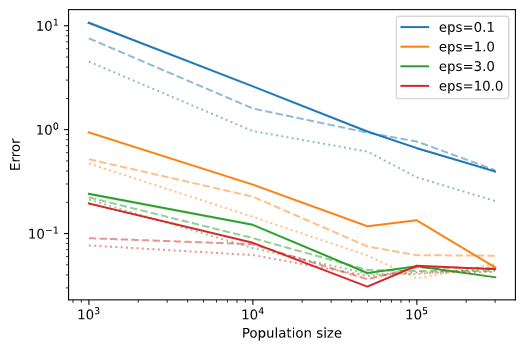
\includegraphics[width=0.6\textwidth]{imgs/histogram_err_normal.png}
                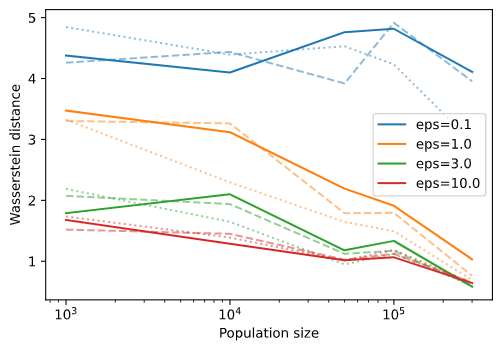
\includegraphics[width=0.6\textwidth]{imgs/histogram_wassersteins_normal.png}}
        }
        \makebox[\textwidth][c]{
            \subcaptionbox{Uniform distribution}
                {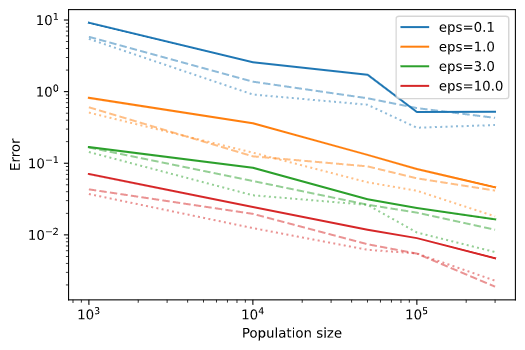
\includegraphics[width=0.6\textwidth]{imgs/histogram_err_uniform.png}
                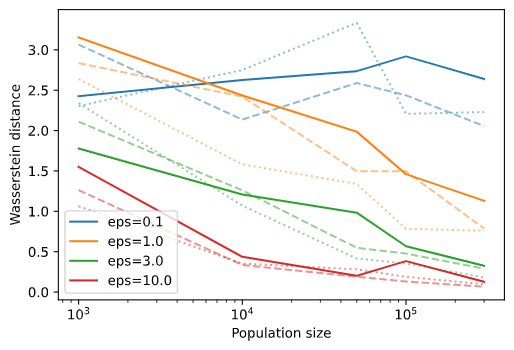
\includegraphics[width=0.6\textwidth]{imgs/histogram_wassersteins_uniform.png}}
        }
        \makebox[\textwidth][c]{
            \subcaptionbox{Constant distribution}
                {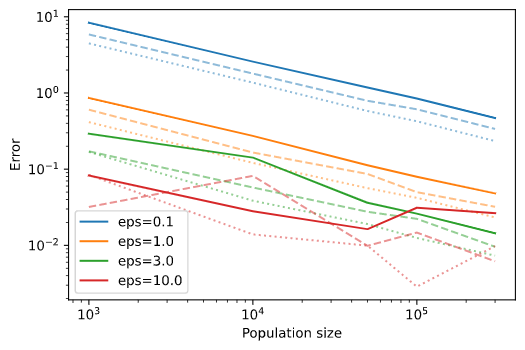
\includegraphics[width=0.6\textwidth]{imgs/histogram_err_constant.png}
                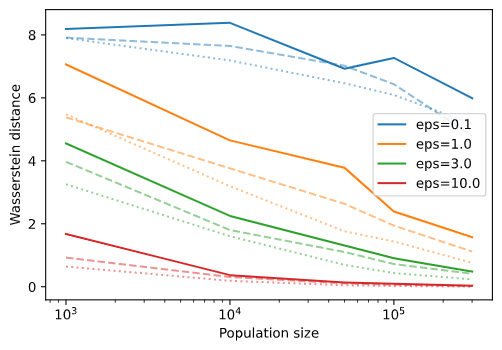
\includegraphics[width=0.6\textwidth]{imgs/histogram_wassersteins_constant.png}}
        }
        \caption{Estimation errors for the histogram estimation mechanism at various $\epsilon$ and population sizes. Solid, dashed and dotted lines are $d=1,2,4$ respectively.}
        \label{fig:histogram_errors}
    \end{figure}
    
    
    
    \begin{figure}
        \centering
        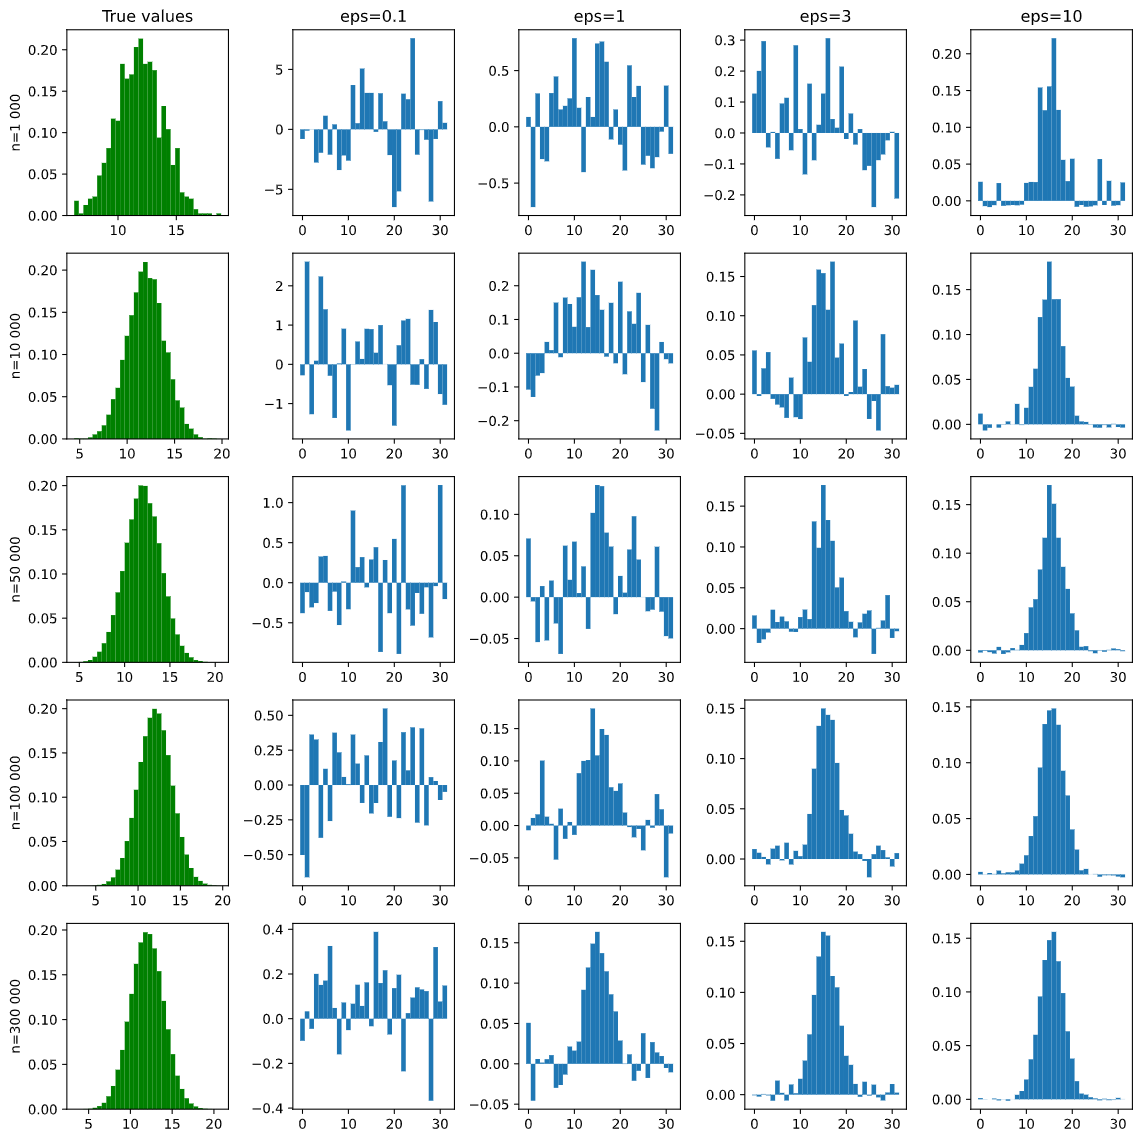
\includegraphics[width=\textwidth]{imgs/histogram_matrix.png}
        \caption{Examples of estimated histograms for various $\epsilon$ and population sizes with $d=1$.}
        \label{fig:histogram_matrix}
    \end{figure}
\end{description}

\subsubsection{Results}

\section{Conclusions}

In this thesis we have explored the topic of differential privacy in chapter \ref{sec:diffpriv}. We have covered its definition and the meaning of the $\epsilon$ parameter. We have covered composition theorems describing the characteristics of combined differentially private algorithms, along with methods for achieving differential privacy for a group of common statistical problems. Finally we have covered common variants of differential privacy, extending the notion to other application areas.

In chapter \ref{sec:telemetry} we have further explored one specific differentially private algorithm. We have experimentally determined its characteristics for small population sizes, an area which was not covered in the original paper. We have applied a formal measure that better describes the distribution estimation capabilities than that used in the paper, and used it to describe the quality of the estimation as $\epsilon$ and population size varies. In particular, we have found that for practical values of $\epsilon$ (e.g. $\epsilon = 3$) the distributions improve significantly even for low population sizes, with the Wesserstein distance nearing 2 at a population size of $10^4$, reaching 1 at $n=10^5$. These results are promising for applications of the algorithm in analytical applications that do not have the user base of Windows 10, which the algorithm was developed for.

\bigskip

Future work may further explore differentially private algorithms; this is a rapidly evolving field, with ample opportunity for further research or literature review. In particular, the application of the memoization techniques from \cite{microsoft_telemetry} on other algorithms in order to extend their privacy guarantees to temporally repeated collection could be an area of interest, as this is a feature often used in telemetry collection.

\printbibliography

\end{document}
